% !TEX encoding = UTF-8
% !TEX TS-program = pdflatex
% !TEX root = ../tesi.tex

%**************************************************************
\chapter{Prodotto}
\label{cap:prodotto}
%**************************************************************

\intro{In questo capitolo viene descritto il prodotto software, la documentazione e i test eseguiti.}\\

%**************************************************************
\section{Prodotto software}
Nel corso di questa sezione vengono descritte tutte le funzionalità implementate al momento del termine dello stage.

\subsection{Login}
Il \textit{login} del prodotto finale dovrà essere gestito tramite un sistema di \gls{ssog} esterno. Nonostante ciò l'implementazione di tale sistema non era tra gli obiettivi dello stage, per la demo finale è stato ritenuto sufficiente utilizzare un \gls{mockg} dello stesso. 
\begin{figure}[h]
    \begin{center}
    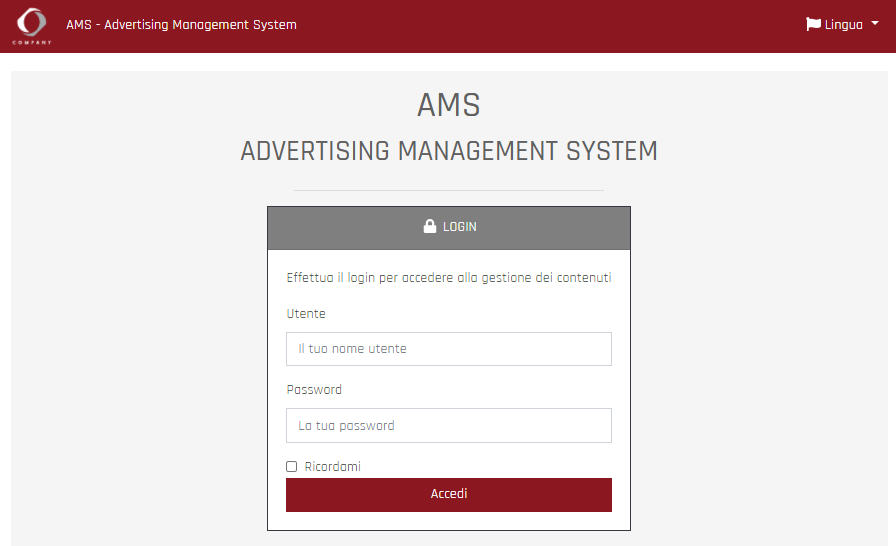
\includegraphics[width=0.95\textwidth]{login}
    \caption{Schermata di login}
    \label{fig:figure20}
    \end{center}
\end{figure}

\subsection{Scelta funzionalità}
La schermata principale del prodotto è la schermata di scelta funzionalità. Tramite questa schermata si possono raggiungere le varie funzioni offerte dal prodotto.
\begin{figure}[h]
    \begin{center}
    
\includegraphics[width=1\textwidth]{funzionalita}
    \caption{Schermata di scelta funzionalità}
    \label{fig:figure21}
    \end{center}
\end{figure}
\\Più nello specifico le funzionalità raggiungibili tramite questa schermata sono:
\begin{itemize}
    \item gestione dei contenuti;
    \item gestione delle campagne (Non abilitata);
    \item visualizzazione \textit{audit}.
\end{itemize}

\subsection{Gestione contenuti}
Tramite la schermata di gestione contenuti è possibile raggiungere le sezioni di lavoro divise per ruolo (Editore, Redattore, Supervisore).
\begin{figure}[h]
    \begin{center}
    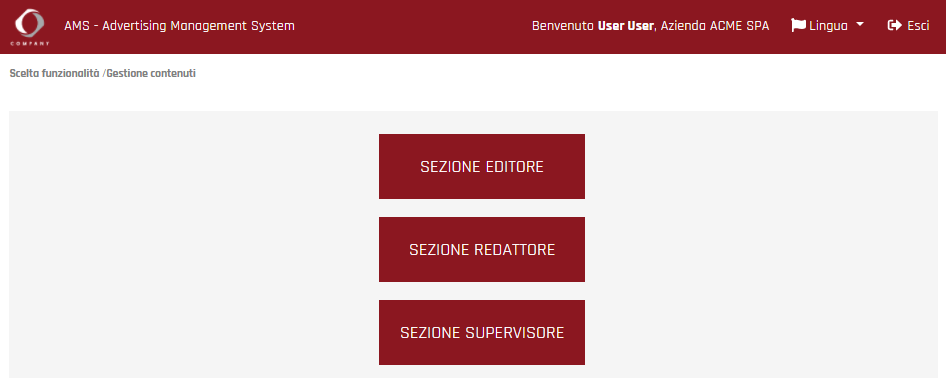
\includegraphics[width=1\textwidth]{gestcont}
    \caption{Schermata di gestione contenuti}
    \label{fig:figure22}
    \end{center}
\end{figure}
\\Ovviamente ogni utente puo visualizzare solamente le sezioni relative ai ruoli a lui assegnati.

\subsection{Sezione editore}
Questa sezione è quella in cui sono utilizzabili la maggior parte delle funzionalità obiettivo dello stage. In questa schermata è visualizzata una lista di tutti i \gls{contenutog}. Per ciascuno di questi è possibile:
\begin{itemize}
    \item visualizzarne l'anteprima;
    \item clonarlo;
    \item modificarlo;
    \item richiederne l'associazione;
    \item eliminarlo.
\end{itemize}
Nel caso sia stata richiesta l'associazione di un contenuto, questo non potra più essere eliminato né modificato.
Tramite questa pagina è inoltre possibile crearne uno nuovo.
\begin{figure}[h]
    \begin{center}
    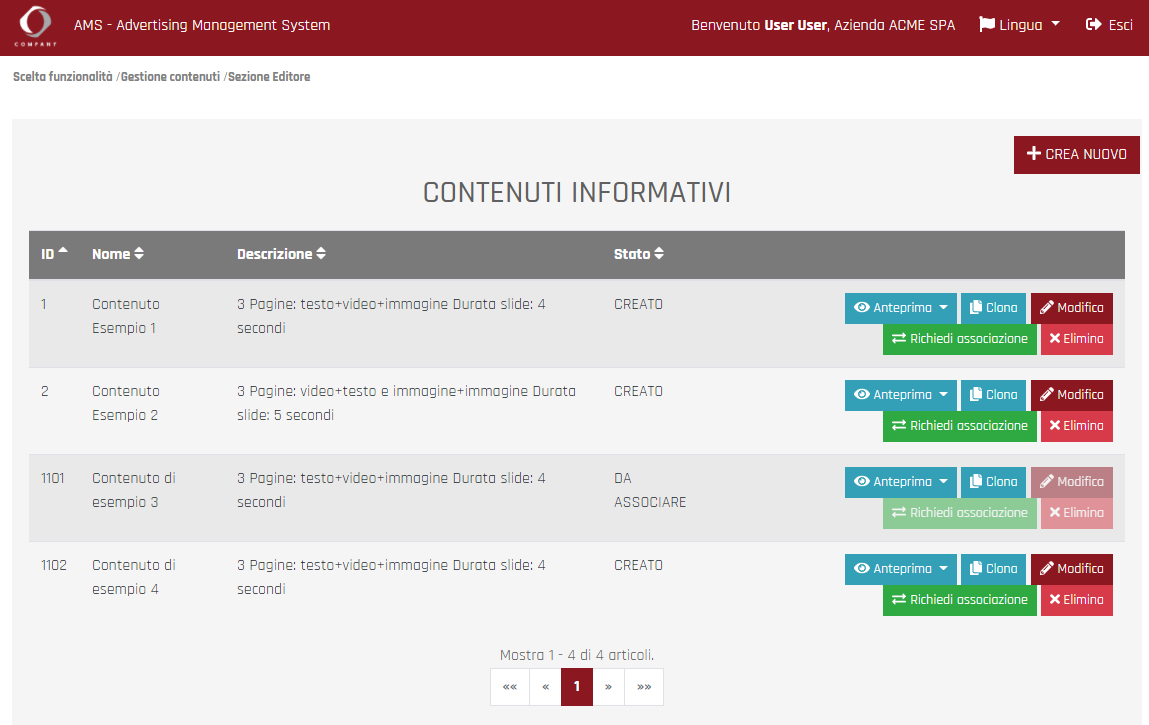
\includegraphics[width=1\textwidth]{editore}
    \caption{Schermata di gestione contenuti}
    \label{fig:figure23}
    \end{center}
\end{figure}

\subsection{Creazione di un contenuto}
La schermate di creazione di un contenuto è divisa in due aree. In quella di sinistra si inseriscono le informazioni generali relative al contenuto. In quella di destra è possibile creare le pagine del contenuto, selezionando per ciascuna uno tra i vari \textit{template} disponibili.
Nel caso si scelgano \textit{template} con contenuti multimediali è sufficiente che questi vengano caricati attraverso l'apposito pulsante. Nel caso ci siano contenuti testuali da inserire è possibile invece utilizzare l'apposito editor di testo.
\begin{figure}[h]
    \begin{center}
    \includegraphics[width=1\textwidth]{Creazione}
    \caption{Creazione di un contenuto}
    \label{fig:figure24}
    \end{center}
\end{figure}

\subsection{Anteprima di un contenuto}
La possibilità di visualizzare l'anteprima di un contenuto una volta creato è una delle funzionalità più utili e importanti. L'anteprima permette infatti di visualizzare come si presenterebbe un contenuto una volta pubblicato e permette di decidere se richiederne l'associazione o modificarlo.
\begin{figure}[h]
    \begin{center}
    
\includegraphics[width=1\textwidth]{anteprima}
    \caption{Anteprima di un contenuto di esempio}
    \label{fig:figure25}
    \end{center}
\end{figure}

\subsection{Clonazione di un contenuto}
La possibilità di clonare un contenuto è utile nel caso si voglia crearne uno simile ad uno già pubblicato senza la necessità di dover partire da zero. Per clonare un contenuto è sufficiente cliccare su \textit{"Clona"} nella sezione dedicata al ruolo di editore. Fatto ciò si aprirà automaticamente un pannello modale in cui è necessario inserire il nome che si vuole assegnare al nuovo contenuto.
\begin{figure}[h]
    \begin{center}
    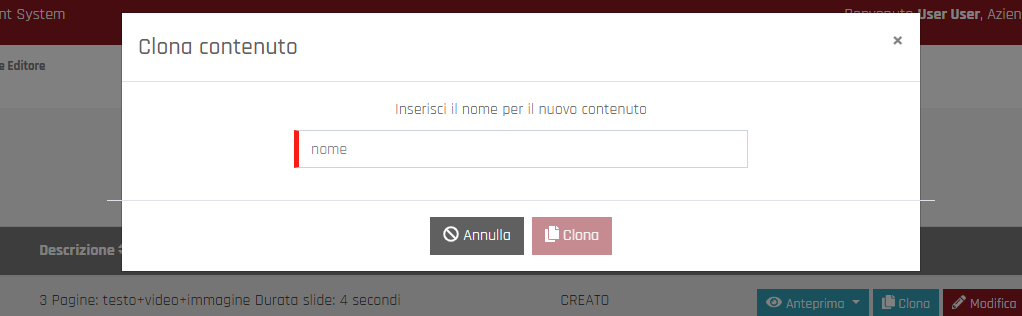
\includegraphics[width=1\textwidth]{clona}
    \caption{Clonazione di un contenuto}
    \label{fig:figure26}
    \end{center}
\end{figure}

\subsection{Modifica di un contenuto}
Modificare un contenuto può essere indispensabile nel caso, ad esempio, siano state inserite immagini o testi errati. La schermata di modifica di un contenuto si presenta in modo analogo a quella di creazione, con la differenza che i campi dati hanno già le informazioni del contenuto al loro interno.
\begin{figure}[h]
    \begin{center}
    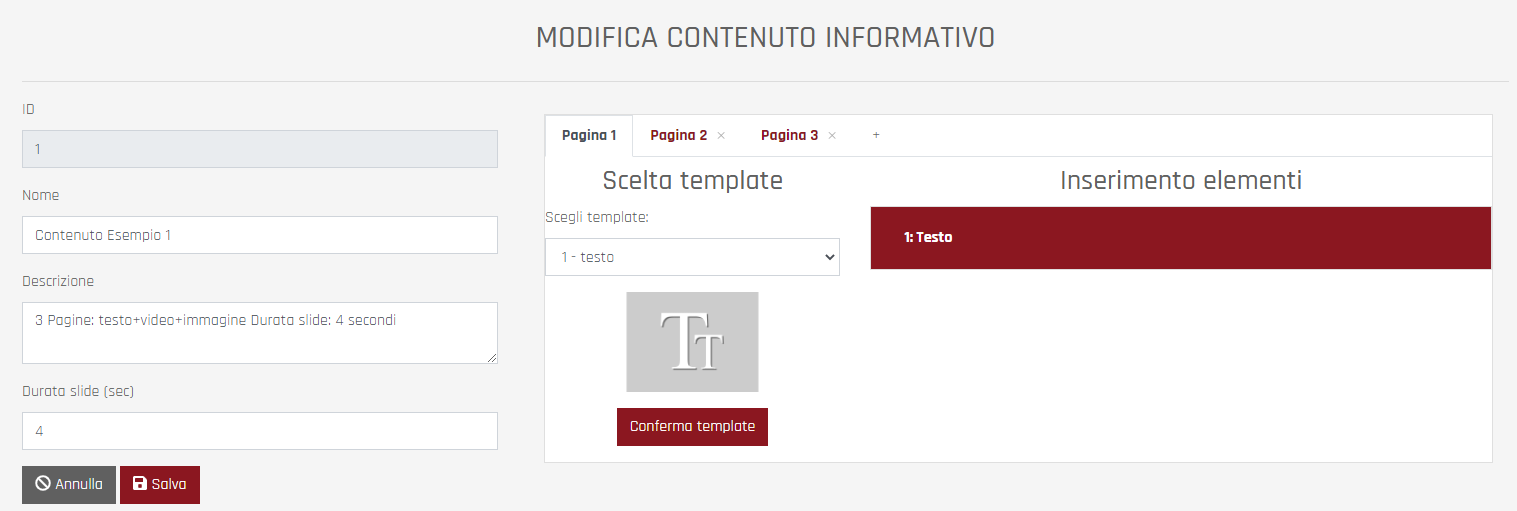
\includegraphics[width=1\textwidth]{modifica}
    \caption{Modifica di un contenuto}
    \label{fig:figure27}
    \end{center}
\end{figure}
\newpage
\subsection{Associazione di un contenuto}
La richiesta di associazione di un contenuto è il primo passo da eseguire perchè questo possa essere pubblicato. Una volta inoltrata la richiesta di associazione di un contenuto questo non potrà più essere modificato ne eliminato. L'associazione può essere approvata o rifiutata da un redattore; nel primo caso il contenuto potrà proseguire nel suo ciclo di vita, nel secondo tornerà allo stato iniziale e sarà di nuovo modificabile.
\begin{figure}[h]
    \begin{center}
    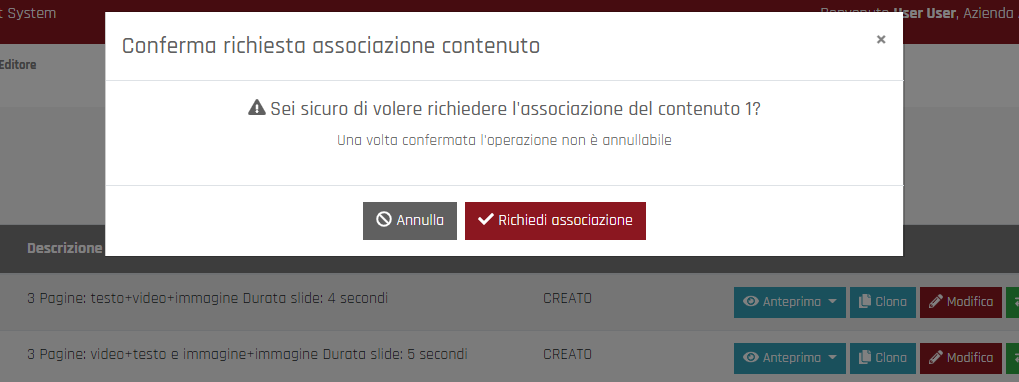
\includegraphics[width=1\textwidth]{associazione}
    \caption{Richiesta di associazione di un contenuto}
    \label{fig:figure28}
    \end{center}
\end{figure}

\subsection{Eliminazione di un contenuto}
Un contenuto potrebbe essere creato per errore oppure non essere più necessario. In questo caso può tornare utile l'eliminazione. L'eliminazione è irreversibile.
\begin{figure}[h]
    \begin{center}
    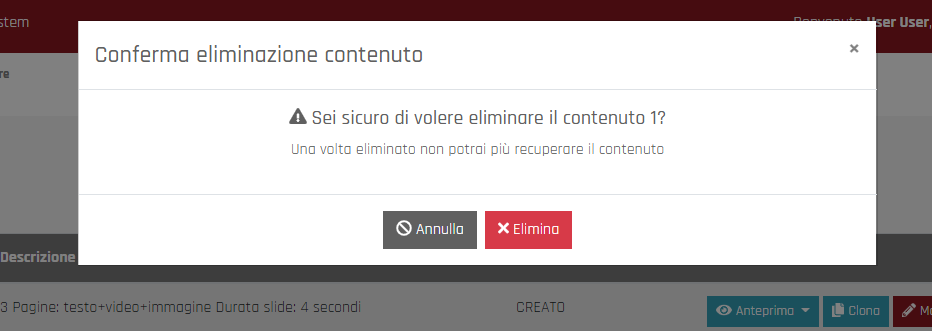
\includegraphics[width=1\textwidth]{eliminazione}
    \caption{Eliminazione di un contenuto}
    \label{fig:figure29}
    \end{center}
\end{figure}

\subsection{Audit}
La schermata di visualizzazione degli \textit{audit}, raggiungibile dalla schermata principale, è visualizzabile da chiunque abbia effetuato il \textit{Login} e raccoglie varie informazioni sulle attività effettuate dagli utenti.
\begin{figure}[h]
    \begin{center}
    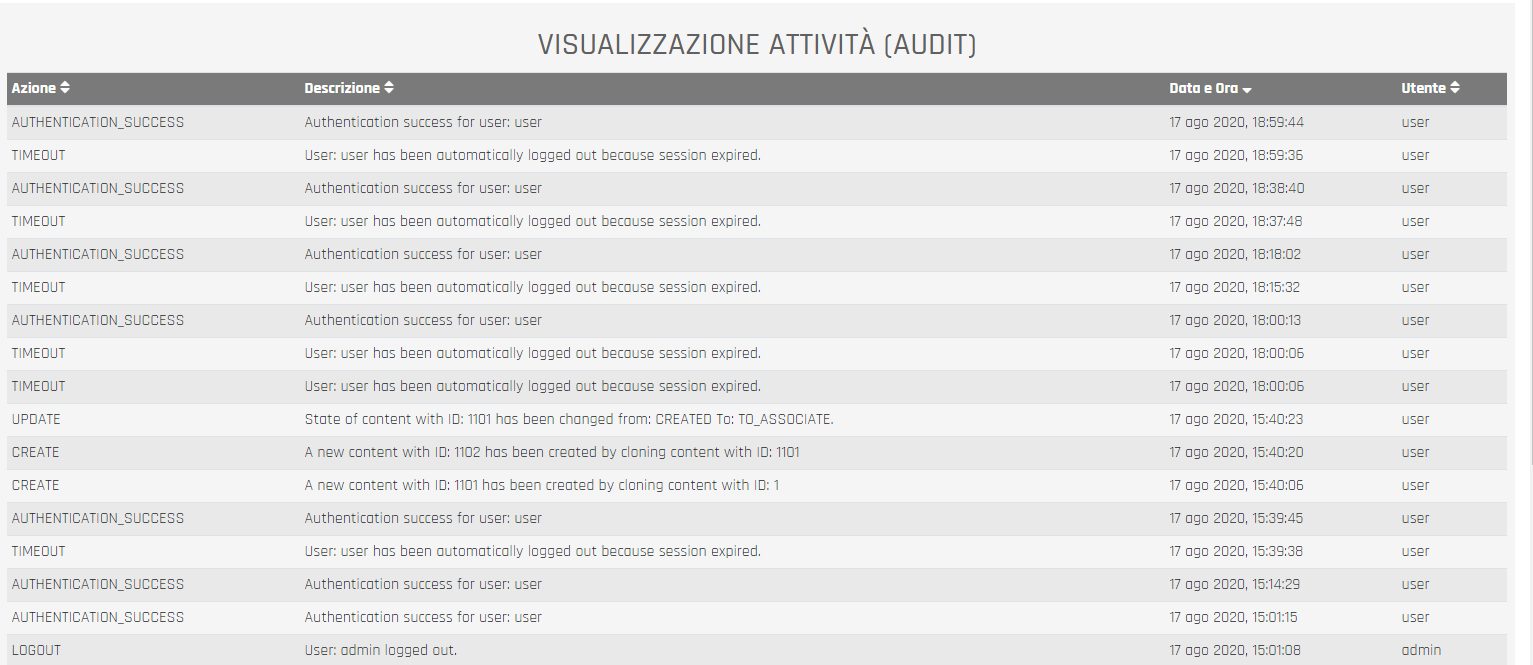
\includegraphics[width=1\textwidth]{audit}
    \caption{Visualizzazione audit}
    \label{fig:figure30}
    \end{center}
\end{figure}

%**************************************************************
\section{Documentazione}
Oltre allo sviluppo dell'applicazione vera e propria, una parte delle ore a disposizione è stata dedicata alla documentazione. In accordo con il \textit{Product Owner} è stato deciso di redigere solamente il manuale utente e il manuale sviluppatore.

\subsection{Manuale Utente}
Lo scopo di questo documento è illustrare tutte le funzionalità del prodotto. In tal modo l'utente finale ha a disposizione tutte le informazioni per utilizzare il \textit{software} correttamente.
Il manuale utente descrive:
\begin{itemize}
    \item requisiti di sistema;
    \item utilizzo dell'applicazione.
\end{itemize}

\subsection{Manuale Sviluppatore}
Lo scopo di questo documento è illustrare le scelte implementative effettuate durante lo sviluppo e dare informazioni utili ad uno sviluppatore che comincia a lavorare a questo progetto.
Il manuale sviluppatore tuttavia non ha lo scopo di sostituirsi alla documentazione ufficiale delle tecnologie utilizzate. Per tale motivo all'interno di esso sono contenuti numerosi riferimenti a documenti esterni.
Il manuale sviluppatore descrive:
\begin{itemize}
    \item setup dell'ambiente di lavoro;
    \item gestione delle dipendenze \textit{Angular};
    \item gestione della dipendenza ad \textit{Oracle};
    \item utilizzo di \textit{Angular CLI};
    \item \textit{build} e \textit{packaging} dell'applicazione;
    \item \textit{testing};
    \item utilizzo di \textit{Docker};
    \item \gls{ci};
    \item scelte implementative effettuate.
\end{itemize}

%**************************************************************
\section{Test}
Nello sviluppo di un'applicazione il \textit{testing} è una delle fasi più importanti. Poiché ogni due settimane veniva presentata una demo dell'applicativo, i \textit{test} sono stati eseguiti di continuo durante lo sviluppo, sia in modo automatico sia manualmente. \\Nel corso di questa sezione vengono descritti i \textit{test} svolti durante lo sviluppo.

\subsection{Test di unità}
I \textit{test} di unità sono eseguiti per verificare se sono presenti errori nei singoli metodi. Nel corso dello stage i \textit{test} di unità sono stati eseguiti tramite \textit{JUnit} e \textit{Jest}. Tali \textit{framework} sono sviluppati rispettivamente per \textit{Java} e per \textit{Javascript}. Il primo è stato utilizzato per testare il \textit{back-end} mentre il secondo per il \textit{front-end}.

\begin{lstlisting}[caption={Test di unità in Java},label={utj}]
    @Test
    @Transactional
    public void createContent() throws Exception {
        int databaseSizeBeforeCreate = contentRepository.findAll().size();
        // Create the Content
        restContentMockMvc.perform(post("/api/contents")
            .contentType(MediaType.APPLICATION_JSON)
            .content(TestUtil.convertObjectToJsonBytes(content)))
            .andExpect(status().isCreated());

        // Validate the Content in the database
        List<Content> contentList = contentRepository.findAll();
        assertThat(contentList).hasSize(databaseSizeBeforeCreate + 1);
        Content testContent = contentList.get(contentList.size() - 1);
        assertThat(testContent.getName()).isEqualTo(DEFAULT_NAME);
        assertThat(testContent.getState()).isEqualTo(DEFAULT_STATE);
        assertThat(testContent.getDescription()).isEqualTo(DEFAULT_DESCRIPTION);
        assertThat(testContent.getSlideTime()).isEqualTo(DEFAULT_SLIDE_TIME);
    }
\end{lstlisting}
\newpage
\begin{lstlisting}[caption={Test di unità in JavaScript},label={utj}]
    describe('Component Tests', () => {
  describe('Home Component', () => {
    let comp: HomeComponent;
    let fixture: ComponentFixture<HomeComponent>;
    let accountService: AccountService;
    let loginModalService: LoginModalService;

    beforeEach(async(() => {
      TestBed.configureTestingModule({
        imports: [AmsTestModule],
        declarations: [HomeComponent],
      })
        .overrideTemplate(HomeComponent, '')
        .compileComponents();
    }));

    beforeEach(() => {
      fixture = TestBed.createComponent(HomeComponent);
      comp = fixture.componentInstance;
      accountService = TestBed.get(AccountService);
      loginModalService = TestBed.get(LoginModalService);
    });

    it('Should call accountService.getAuthenticationState on init', () => {
      // WHEN
      comp.ngOnInit();

      // THEN
      expect(accountService.getAuthenticationState).toHaveBeenCalled();
    });

    it('Should call accountService.isAuthenticated when it checks authentication', () => {
      // WHEN
      comp.isAuthenticated();

      // THEN
      expect(accountService.isAuthenticated).toHaveBeenCalled();
    });

    it('Should call loginModalService.open on login', () => {
      // WHEN
      comp.login();

      // THEN
      expect(loginModalService.open).toHaveBeenCalled();
    });
  });
});
\end{lstlisting}

\subsection{Test di integrazione}
I \textit{test} di integrazione vengono eseguiti per verificare che non ci siano errori di integrazione tra le varie componenti del sistema. Nel corso del progetto questa fase di \textit{test} è stata ritenuta di grande importanza, in particolare nell'integrazione tra il \textit{back-end} e il \textit{front-end}. In questo caso i suddetti \textit{test} sono stati eseguiti manualmente. 

\subsection{Test di sistema}
I \textit{test} di sistema vengono eseguiti per assicurare che il sistema soddisfi i requisiti richiesti. \\Nel corso dello stage dopo l'implementazione di una nuova funzionalità l'intero sistema veniva testato. Al termine di ogni sprint tali \textit{test} venivano eseguiti dal \textit{product owner}, in tal caso questi possono essere considerati \textit{test} di accettazione.

\subsection{Test di performance}
I \textit{test} di performance vengono eseguiti per controllare che il sistema non risulti lento durante il suo utilizzo. Tali \textit{test} sono stati eseguiti con l'ausilio del pannello amministratore generato da \textit{JHipster}. Questo permette di visualizzare una moltitudine di informazioni, come ad esempio le risorse occupate o il tempo di esecuzione delle \gls{apig}.
\begin{figure}[h]
    \begin{center}
    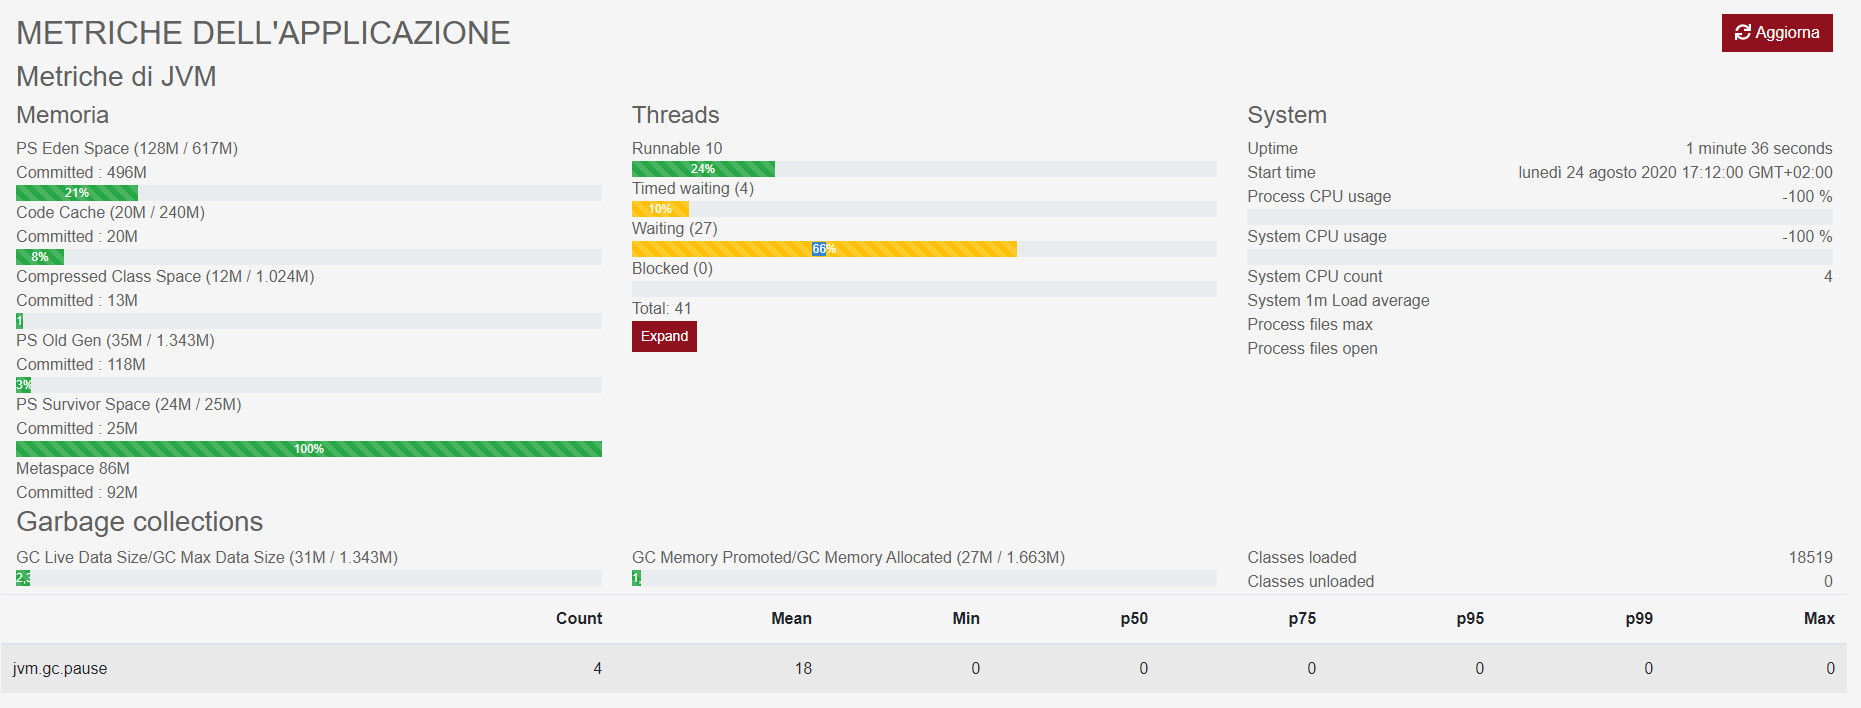
\includegraphics[width=1\textwidth]{metriche1}
    \caption{Metriche dell'applicazione}
    \label{fig:figure31}
    \end{center}
\end{figure}

\section{Accessibilità}
I \textit{test} di accessibilità sono necessari per verificare che l'applicativo risulti utilizzabile anche da utenti con disabilità. Nel corso del progetto si è cercato di attenersi alle regole definite nello standard \href{https://www.w3.org/TR/WCAG21/}{WCAG 2.1}. I test veri e propri sono stati poi eseguiti tramite \href{https://developers.google.com/web/tools/lighthouse/?utm_source=devtools}{\textit{Lighthouse}}, un tool per l'analisi dinamica di pagine web.